\section{Experiments}\label{sec:experiments}


We evaluate the proposed instance- and time-adaptive conformal framework on four multivariate time-series forecasting benchmarks.

\label{sec:experimental_setup}
\textbf{Datasets.}
We evaluate our method on 
%two widely used time series forecasting datasets~\cite{autoformer}: 
%ETTh1 and ETTm1.
four Electricity Transformer Temperature (ETT) datasets (ETTh1, ETTh2, ETTm1, ETTm2)~\cite{informer}.
%Exchange~%\cite{lai2018modeling} and Illness (ILI)\footnote{
%https://gis.cdc.gov/grasp/fluview/fluportaldashboard.html}.



\textbf{Experimental Protocol.} Our experiments follow the standard protocol used in recent time series forecasting literature \cite{Yuqietal-2023-PatchTST,liu2023itransformer, wang2024deep}. For  all datasets, we use a forecast horizon length $h \in \{96,192,336,720\}$. A look-back window of 96 is used for all experiments. 

\textbf{Implementation and Training Details.}
 We used a standard transformer-based state-of-the-art expert model: iTransformer \cite{liu2023itransformer}. It is available from the Time Series Library (TSLib)~\cite{wang2026deep}, with an uncertainty estimation head, as detailed in Section 2.  We trained all models using the Adam optimizer for a maximum of 10 epochs, with early stopping patience set to 3 epochs. The learning rate was set to $\lambda=0.001$. All experiments were conducted on a single NVIDIA A100 80GB GPU. By default, all MoGE configurations utilize three experts, unless otherwise specified.
To handle non-stationarity, we used a sliding calibration window of 1000 scores, initialized from the validation set, and set the ACI parameter to $\delta=0.001$ \cite{gibbs2021adaptive}. Calibration is performed independently for each channel and forecast horizon.
%{\bf Rolling calibration.} Time-series data are neither stationary nor exchangeable, so a fixed calibration set becomes stale as the data distribution drifts. 
%In all our experiments, w



\begin{table}[t]
  \caption{ACI-adapted calibration intervals at a $0.90$ target coverage, ETT datasets, aggregated over 5 training seeds as mean $\pm$ sample standard deviation.  Bold marks the narrowest mean width. }
  \label{tab:ett_aci} 
  \vspace{0.1cm} 
           \scalebox{0.8}{
  \begin{tabular}{l  l  r r}
  \hline
   \textbf{Dataset} &  \textbf{Calibration} & \textbf{Coverage} $\uparrow$ & \textbf{Avg. Width} $\downarrow$ \\

  \hline
  \multirow{5}{*}{ETTm1}   &CP-MoG   & $0.901 \pm 0.000$ & $\mathbf{1.670 \pm 0.030}$ \\*
         & CP-MoG-a & $0.901 \pm 0.001$ & $1.672 \pm 0.029$ \\*
    & CP-G  & $0.901 \pm 0.000$ & $1.704 \pm 0.017$ \\
     & CQR  & $0.899 \pm 0.002$  & $2.774 \pm 0.215$ \\*
     & CQR (retrained) & $0.899 \pm 0.001$ & $1.985 \pm 0.059$ \\
  \hline
  \multirow{5}{*}{ETTm2} &  CP-MoG   & $0.900 \pm 0.000$ &$\mathbf{ 1.538 \pm 0.059}$ \\*
       & CP-MoG-a & $0.900 \pm 0.001$ & $1.540 \pm 0.059$ \\*
      & CP-G  & $0.901 \pm 0.000$ & $1.647 \pm 0.072$ \\*
       & CQR  & $0.890 \pm 0.007$ & $3.943 \pm 0.763$ \\*
     & CQR (retrained)  & $0.897 \pm 0.001$ & $2.209 \pm 0.605$ \\
      \hline
  \multirow{5}{*}{ETTh1} & CP-MoG  & $0.898 \pm 0.001$ & $\mathbf{1.740 \pm 0.004}$ \\*
  & CP-MoG-a & $0.898 \pm 0.001$ & $1.741 \pm 0.004$ \\
     & CP-G  & $0.898 \pm 0.001$ & $1.762 \pm 0.011$ \\*
        & CQR & $0.894 \pm 0.009$ & $3.786 \pm 0.168$ \\*
     & CQR (retrained)  & $0.886 \pm 0.007$ & $2.511 \pm 0.228$ \\
  \hline
  \multirow{5}{*}{ETTh2}  &CP-MoG   & $0.892 \pm 0.001$ & $\mathbf{1.875 \pm 0.036}$ \\*
     & CP-MoG-a & $0.893 \pm 0.001$ & $1.880 \pm 0.035$ \\*
   &  CP-G   & $0.892 \pm 0.001$ & $1.896 \pm 0.066$ \\
 
     & CQR  & $0.886 \pm 0.009$ & $4.460 \pm 0.271$ \\*
     & CQR (retrained) & $0.883 \pm 0.011$ & $3.233 \pm 0.644$ \\
     \hline
   \end{tabular}
   }
\end{table}



\textbf{Evaluation measures.} The standard way to evaluate the performance of confidence-interval estimators on a given test set $(x_1,y_1),...,(x_n,y_n)$ is by computing the degree of coverage and the average length of the prediction intervals.   Smaller average interval widths indicate higher precision.  The length and coverage are formally defined as:
$$ \textrm{length} = \frac{1}{n} \sum_i | C(x_i) |,
\hspace{0.2cm}  \textrm{coverage} = \frac{1}{n} \sum_i 
{\textbf 1}(y_i \in C(x_i))$$
such that $C(x_i)$ is the confidence interval of  $x_i$  and $|C(x_i)|$ is its length.
The best algorithm is the one that reports the minimal average interval length among those that satisfy the coverage requirement. We report CP results across five random initializations (seeds) of the time-series prediction model.   

%\begin{figure}[htbp]
 %   \centering
  %%  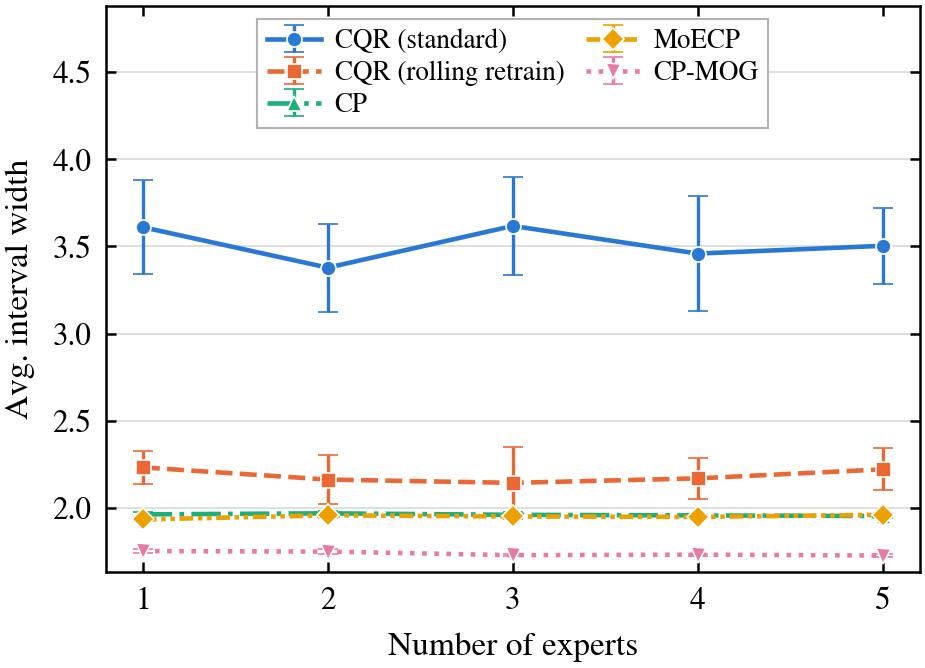
\includegraphics[width=\columnwidth]{avg_width_vs_experts_ETTh1.png}
   % \caption{Average width of the $90\%$ prediction intervals on ETTh1 (iTransformer, horizon $96$) vs.\ the number of experts; mean $\pm 1$ s.d.\ over five seeds.}
    %\label{fig:avg_width_experts_etth1}
%\end{figure}


{\bf Compared methods.} 
We implemented several CP frameworks to generate instance-dependent prediction intervals.
CP-MoG is based on calibrating the total variance and CP-MoG-a is based on calibrating the within-expert part of the variance. 
CP-G is based on calibrating the variance of a single Gaussian model.
We also implemented two variants of  CQR \cite{cqr2019}. CQR requires training a quantile regression network and calibrating its results.
In the first variant (denoted CQR(retrained)), we trained a new QR network for each sliding window and in the second variant, we used a fixed QR network and recalibrated it for each sliding window.


{\bf Results.} Table \ref{tab:ett_aci} summarizes the calibration results, showing that the average interval width (Avg. Width) obtained by
CP-MoG is substantially smaller than that achieved by CQR. The reported empirical coverage values are close to the target level of $90\%$ in almost all cases.
The strong performance obtained even with a single-Gaussian uncertainty model demonstrates that the benefit of the proposed framework is not specific to mixture-of-experts architectures. MoGE provides an additional improvement by offering a richer estimate of predictive uncertainty.
 We observe that even a single-Gaussian model yields considerably better results than CQR. Using multiple experts further improves the results. In the case of MoGE, we did not observe a significant difference between using the total variance and using only the within-expert component. 
 The nearly identical performance of CP-MoG and CP-MoG-a suggests that, for these datasets and prediction models, the within-expert component dominates the predictive variance.
To quantify this, we compute the ratio of the aleatoric to the epistemic variance component, $\mathbb{E}[\sigma_a^2(x)] / \mathbb{E}[\sigma_e^2(x)]$, pooled over all test points and all five seeds: $216$ on ETTh1, $72$ on ETTh2, $163$ on ETTm1, and $189$ on ETTm2. The aleatoric term therefore dominates the total predictive variance by roughly two orders of magnitude on every dataset, which explains why CP-MoG and CP-MoG-a perform nearly identically.
We further assess how informative the total predicted variance $\sigma_a^2(x)+\sigma_e^2(x)$ is about the realized squared error $(y-\hat{y}(x))^2$ via their Pearson correlation, again pooled over all test points and seeds. The correlation is substantially higher on ETTh1 ($r=0.435$) and ETTm1 ($r=0.339$) than on ETTh2 ($r=0.132$) and ETTm2 ($r=0.114$), indicating that the variance head is more informative about instance-level forecast difficulty on ETTh1/ETTm1 than on ETTh2/ETTm2.
   The fixed CQR model generally produces substantially wider intervals and, in the case of ETTm1, also exhibits considerable undercoverage. Retraining the QR model for each window improves its performance, but at the cost of substantially higher computational complexity.
  At comparable coverage, CP-MoG reduces the average interval width by approximately 40–60\% relative to CQR across the four ETT datasets.


